\chapter{Background}
\label{sec:background}
\minitoc
\vspace*{1cm}

In this chapter, we provide background information giving a detailed understanding of several key points about this thesis. First, we define what a Cross-Site Scripting bug is in web applications by giving specific examples of how this vulnerability may occur. Then, we briefly discuss what fuzzing is and the various categories that constitute it, showing how \emph{instrumentation} helps when used during grey-box fuzzing. Towards the end, this chapter discusses the concept of concurrency in Python and concludes with the containerization of services using Docker.

\section{Web Application Bugs}
The internet has been growing exponentially since its commercial inception in 1969 with the creation of ARPANET. Although there are over 1 billion pages currently online, writing a web application secure from any vulnerability can be extremely difficult. Every significant web application, especially large-scale ones that are composed of thousands of Lines of Code (LoC), have dangerous bugs in them. Popular social-networking site Facebook had bugs in its 100 million LoC that resulted in 50 million users having their personal data exposed ~\cite{facebook_data_breach,facebook_loc}. Such problems are not exclusive to complex web applications. Even the simplest web-apps can be the root of irreparable damage when they are exploited by attackers with ulterior motives. 

In fact, web application vulnerabilities are among the most frequent vulnerabilities reported in the Common Vulnerabilities and Exposures database (CVE). According to CVE 2019 data, Denial of Service  (DoS) (19.2\%) is ranked second and Cross-Site Scripting (XSS) (12.5\%) is fourth among the top Cybersecurity vulnerabilities ~\cite{cve}.

The Open Web Application Security Project (OWASP) Top 10 represents a broad consensus on the most critical security risks to web applications ~\cite{owasp2017}. One of the most pressing security issues on the Internet, according to the OWASP list, is Cross-Site Scripting (ranked 7).

XSS flaws occur whenever an application includes untrusted data in its web page responses without validating or escaping them first. In other words, the web application accepts input from the user and then attempts to display it without filtering for HTML tags or script code, such as JavaScript. JavaScript is an essential part of web applications as it is used during both frontend and backend development with all major web browsers having a dedicated engine to execute {\tt .js} code. So, allowing such untrusted code to be executed can hijack the browser, deface the website, redirect the user to dangerous sites and many other attacks. Some XSS types include Reflected (Non-Persistent or Type II), Stored (Persistent or Type I) and DOM-based (Type-0).

Reflected XSS ~\cite{rxss_def} vulnerabilities arise when arbitrary data is copied from a request and echoed into the application's immediate response. By not filtering the data input, scripting language code included within a request can be executed, whatever its content. In the case of Stored XSS vulnerabilities, the malicious payload is permanently stored in storage such as a database residing on a server and is only later outputted by an unsuspecting query. Locations, where Stored XSS may occur, include Web forums or blog comments. 

\pname{} focuses on detecting bugs that can lead to both Reflected or Stored Cross-Site Scripting, that are among the most common of XSS attacks. A step-by-step illustration of the latter can be seen in Figure ~\ref{fig:storedxss} and the former in Figure ~\ref{fig:reflectedxss}. In both illustrations, the attacker and victim are represented by \pname{}.

It is imperative that we understand what an RXSS (Reflected XSS) bug typically looks like, in order to grasp the thesis' perspective on such vulnerabilities. Usually, RXSS is caused due to a failure to sanitise user input. For instance, let us assume that we have a simple login page with two input fields: the username and password. The login page also displays the appropriate error messages back to the user if the login fails. An implementation of this in PHP could look something like Listing ~\ref{lst:vuln_login_sub}.

\begin{lstlisting}[aboveskip=\baselineskip, showstringspaces=false, frame=single, language=PHP, caption={\textit{Vulnerable login form}}, numberstyle=\color{gray}, numbersep=5pt, label={lst:vuln_login_sub}]
<?php
$username=$_POST['username'];
$pwd=$_POST['password'];
if (search_username($username)) {
   if (match_username_password($username, $pwd)) {
      // do normal login procedures
   } else {
      echo 'Wrong Password';
   }
} else {
      echo 'Error' . $username . 'was not found.';
}
?>
\end{lstlisting}

\begin{figure}[ht]
 \centering
 \captionsetup{justification=centering}
 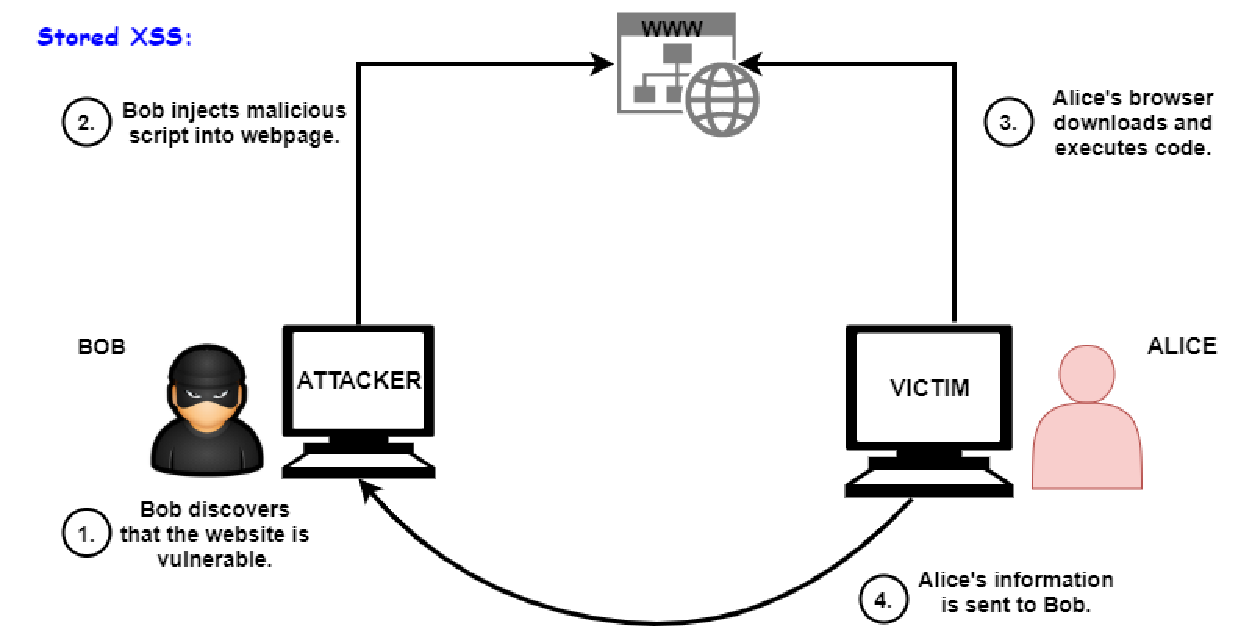
\includegraphics[width=\linewidth]{figures/storedxss.pdf}
 \caption[How Stored Cross-Site Scripting can be exploited by an attacker]{\textit{How Stored Cross-Site Scripting can be exploited by an attacker}}
 \label{fig:storedxss}
\end{figure}

\begin{figure}[ht]
 \centering
 \captionsetup{justification=centering}
 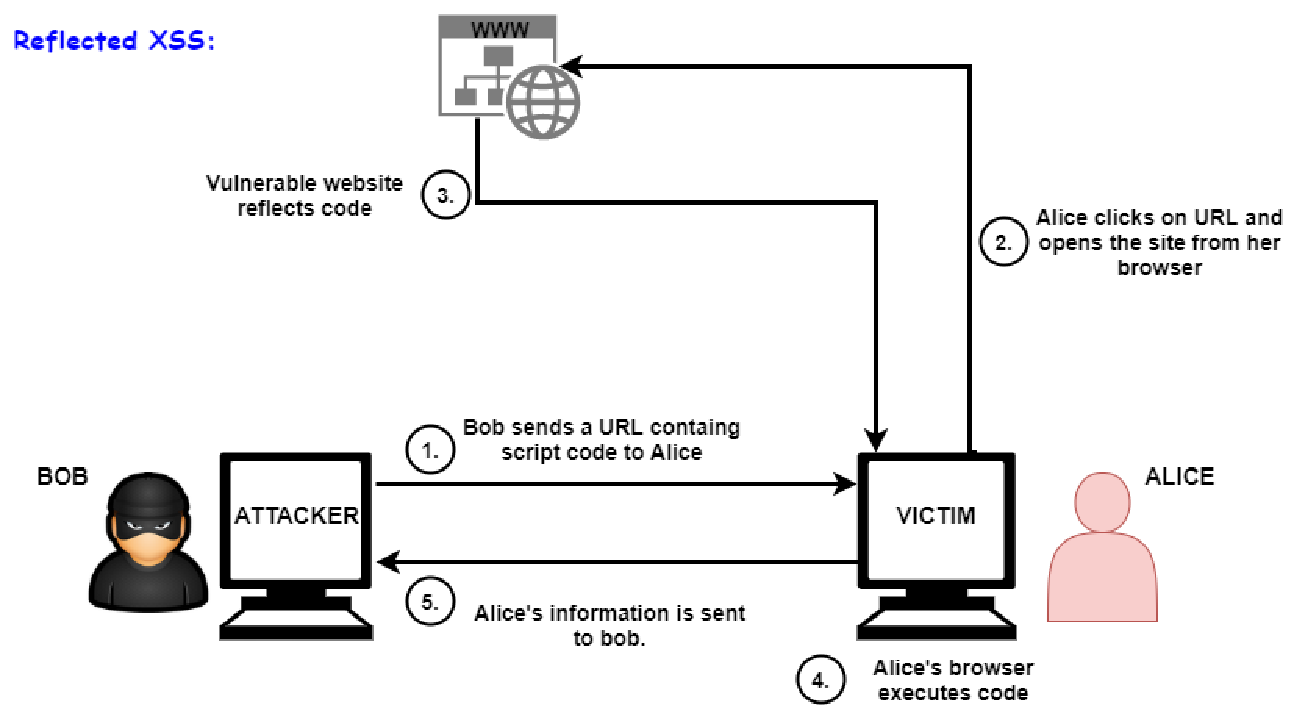
\includegraphics[width=\linewidth]{figures/reflectedxss.pdf}
 \caption[How Reflected Cross-Site Scripting can be exploited by an attacker]{\textit{How Reflected Cross-Site Scripting can be exploited by an attacker}}
 \label{fig:reflectedxss}
\end{figure}

The above code is faulty for two reasons. First, knowing a username exists offers clues for an attacker to guess a set of correct credentials much faster since only the password is left to find. But this design choice is not linked with Cross-Site Scripting. The source of the bug is on line 11 where the error message "{\tt the \$username was not found}" is displayed. Because {\tt \$username} is a variable that has not been sanitized, an attacker can inject malicious payload in this field that will be interpreted by the HTML parser according to whatever its content is. 

{\tt Exploit:} A victim is tricked into submitting a {\tt form} located in an attacker-controlled website. The malicious payload is designed to trigger the vulnerability found in the above login {\tt form} (Listing ~\ref{lst:vuln_login_sub}). As soon as the {\tt form} is submitted, the vulnerable login page is opened with the XSS script executed in it. When the victim tries to login, the XSS script can easily send the credentials to the attacker as well. 

Another example of a vulnerable page is highlighted in Appendix ~\ref{sec:appendixc}. This presents a more complex scenario than the one shown in Listing ~\ref{lst:vuln_login_sub}, since a \emph{magic number} must be guessed first before entering a conditional branch to reach the XSS vulnerability.

Defeating XSS attacks is not dissimilar to defending against other types of code injection.
The input must be sanitized. User input containing HTTP code must be escaped or encoded to avoid its execution. System-wide measures such as Content Security Policy (CSP) ~\cite{csp_def} may be enabled to eliminate or mitigate XSS attacks. Nevertheless, flaws such as Buffer Overflows (CVE ranked 3 ~\cite{cve}) or Cross-Site Scripting issues comprise a majority of security incidents that malicious hackers exploit daily. 

\section{Fuzzing}
A promising method for discovering unknown vulnerabilities in programs and web applications proven to be very effective, is a technique called fuzzing (or fuzz testing) ~\cite{fuzzing_def}. Fuzzing was invented by Barton Miller at the University of Wisconsin, as one of several tools to test UNIX utilities ~\cite{mller1990fuzz}. With this quality assurance technique, the software is exercised using a vast number of anomalous inputs for inferring if any of them introduce security-related side-effects. A fuzzer, the tool that automates the aforementioned stress-testing process can be categorized in relation to its awareness of the program structure as black-, white-, or grey-box ~\cite{fuzzing_book}. 

A black-box fuzzer treats the program as a 'black box' and is unaware of internal structures. It conducts its test on the target through external interfaces and produces random inputs using no information about the target's underlying structure. More often than not, black-box fuzzers are only able to scratch the surface and expose "shallow" bugs ~\cite{fuzzing_owasp}. For example, the branch of the conditional statement "{\tt if x==5:}" has only one in $2\textsuperscript{32}$ chance of being executed if {\tt x} is a randomly chosen 32-bit input value (\ie an integer). That intuitively explains why black-box testing usually provides low code coverage and is unable to find bugs nestled deep in the program ~\cite{Godefroid2008AutomatedWF}.

A white-box fuzzer infers source code knowledge, such as source code auditing, to reveal
flaws in the software. It leverages program analysis to systematically
increase code coverage or to reach certain critical program locations otherwise unreachable. Program analysis can be based on either static or dynamic analysis, or their combination ~\cite{program_analysis_book}. They may also leverage symbolic execution to derive what inputs cause each part of a program to execute ~\cite{king1976symoblic}. It makes them effective at exposing bugs that hide deep in the program. By studying the application code, you can detect optional or proprietary features, which should be tested as well.

A fuzzer is considered grey-box when it leverages \emph{instrumentation} rather than program analysis to glean information about the coverage of a generated input from the program it tries to fuzz ~\cite{zalewski2015american,efs2007}. Adopting this process significantly reduces the 'guesswork' that occupies black-box fuzzers. This thesis explores in detail grey-box fuzzing, which combines elements of the white-box and black-box approaches since it uses the internals of the software, to a minimal extent, to help generate better test cases without needing full access to the code. 

We also explored the feasibility of constructing a fuzzing tool that will automate the process of discovering bugs in web applications. This was done by providing randomized invalid inputs to an under-analysis instrumented web application, mutating these inputs according to the feedback received and finding test cases that cause a systems crash or make them act inappropriately to prevent exploitable vulnerabilities.

\section{Instrumentation}
Typically, a fuzzer is considered more effective if it achieves a higher degree of code coverage. To be able to trigger any given bug, the fuzzer must first execute the code where the bug lies. So, widening code coverage increases the chances of executing unsafe pieces of code where bugs may reside. As mentioned in the previous section, using \emph{instrumentation} may be the key to achieving a higher code-coverage percentage. 

However, some studies have failed to reach a consensus on the correlation between code coverage and the number of bugs found ~\cite{klees2018Evaluation,coverage2014effectiveness}. 
Increasing global code coverage may be less effective in finding new bugs than, for instance, focusing on widening code coverage in targeted error-prone code areas as AFLGo ~\cite{bohme2017directed} does. Therefore, code coverage should be considered a secondary metric and the number of bugs found as the primary ~\cite{klees2018Evaluation}. Nevertheless, measuring coverage is crucial for any fuzzer.

Available fuzzers for web applications act in a black-box fashion~\cite{doupe2010johnny}; by applying brute force to the target with URLs that embed known web-attack payloads with little or no information about the underlying structure of the target. In contrast, \pname firstly instruments a web application by adding code that tracks all control flows triggered by an input and notifies the fuzzer, accordingly. Notifications can be embedded in the web application's HTTP response using custom headers or it can be outputted to a shared file or memory region. 

Consequently, the fuzzer sends requests to the target and analyses the responses to detect any requests of interest that would later help to improve the code coverage and as a result, trigger vulnerabilities nested deep in the web application's code. To measure code coverage we calculate the ratio of how many basic blocks were visited in respect to the total number of basic blocks instrumented. It gives us a good idea of the coverage but omits information such as sequences of basic blocks that were visited.

We instrumented web applications for delivering feedback once being fuzzed. As opposed to native applications, where several options exist for instrumenting their source or binary representation. We decided to instrument web applications by modifying the AST of PHP files and then reverting it to source code form. This provided us with crucial feedback on the basic blocks that are visited during the analysis. \emph{Instrumentation} performed by \pname on our targeted web application is similar to how AFL instruments binaries, but adapted to work in web applications.

\section{Concurrency}
Concurrency is defined as working on multiple tasks at the same time ~\cite{concurrency_realpython}. However, in Python this does not mean that they work in parallel, since only one core of the CPU is active at any given time. Instead, each task takes turns in occupying the core and executing their code. When a task is interrupted, its state is stored so it can restart from the point where it left off. 

Concurrency aims to speed up the overall performance of input/output (I/O) bound programs, whose performance can be slowed dramatically when they are obliged to frequently wait for I/O operation from an external resource. An example of such resources are requests over the internet or any type of network traffic that takes several orders of magnitude longer than CPU instructions. An illustration of the above can be seen in Figure ~\ref{fig:concurrency_example}:

\begin{figure}[ht]
 \centering
 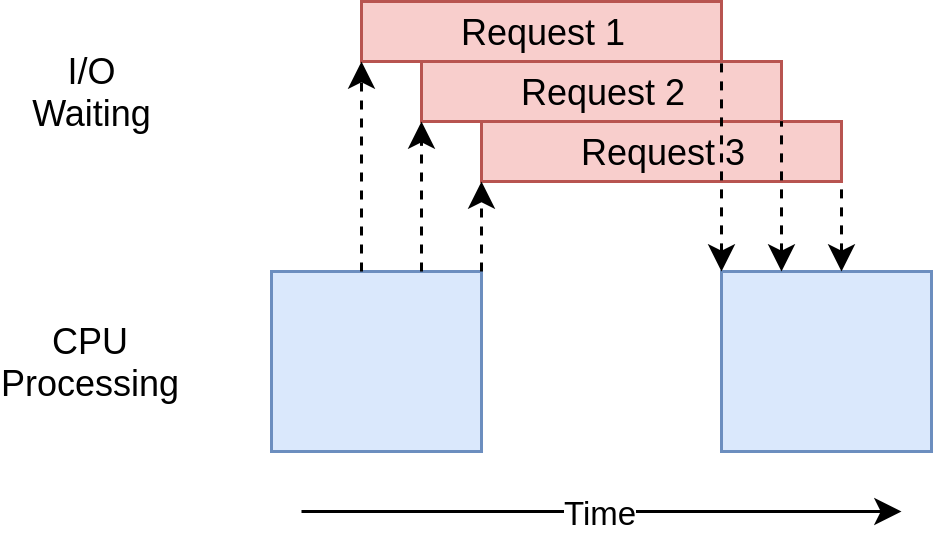
\includegraphics[width=\linewidth]{figures/concurrency_example.png}
 \caption[Requests over the internet processed concurrently]{\textit{Requests over the internet processed concurrently} ~\cite{concurrency_realpython}}
 \label{fig:concurrency_example}
\end{figure}

In Python, concurrency is expressed either through the Threading or AsyncIO (short for Asynchronous Input Output) ~\cite{asyncio} modules. Due to the infamous \emph{Global Interpreter Lock} (GIL) ~\cite{gil_realpython} Python has, both AsyncIO and Threading, they are single-threaded, single-process design. There was no clear advantage in using the latter so, AsyncIO was opted for instead, although initial work was done with {\tt threading} it was shelved. Not to mention the added complexity of using threads and making the program thread-safe. 

Briefly, GIL ensures there is only one thread running at any given time, thus making the use of multiple cores/processors with threads infeasible. In the Python community there is a general rule of thumb when it comes to I/O-bound problems; "Use asyncio when you can, threading when you must". More information on the AsyncIO module and its use in the \pname implementation can be found in Chapter ~\ref{sec:implementation}.

\section{Docker}
Docker containers ~\cite{docker_containers} provide developers the commodity for creating software locally with the knowledge that it will run identically regardless of the host environment ~\cite{using_docker_book}. Containers are an encapsulation of an application's dependencies that share resources with the host OS, unlike frequently used \emph{Virtual Machines}. During the evaluation, detailed in Chapter ~\ref{sec:evaluation}, a docker-compose {\tt YAML} file was created to allow multiple containers to be initiated and managed at the same time with a set of pre-defined configurations. 

Services are deployed with containers through the use of Docker images. A Docker image consists of a collection of files that bundle together all the essentials, such as installations, application code and dependencies required to configure a fully operational container environment. Official Docker images can be found at Docker Hub ~\cite{docker_hub}.